\documentclass[11pt,a4paper]{ivoa}
\input tthdefs

\usepackage{array}
\usepackage{tabulary}  % for nicer tables
\usepackage{calc}
\usepackage{placeins}
\setlength\extrarowheight{2pt}

\newcolumntype{L}{>{\centering\arraybackslash}m{3cm}}

\title{Model Instances in Votables}

% see ivoatexDoc for what group names to use here
\ivoagroup{DM}

\newcommand{\TODO}[1]{%
    \noindent%
    \colorbox{todocolor}{%
            \parbox{0.85\linewidth}{\sffamily \textbf{TODO:}\\
            #1}
    }%
    \vspace{2pt}
}

\newcommand{\note}[1]{%
    \noindent%
    \textcolor{darkgrey}{{\sffamily Note:} \emph{#1}}%
}

\newcommand{\comment}[1]{%
    \noindent%
    \textcolor{red}{{\sffamily Comment:} \emph{#1}}%
}

%%%%%%%%%%%%%%%%%%%%%%%%%%%%%%%%%%%%
% XML syntax coloration and formatting
%
\definecolor{todocolor}{rgb}{1,1,0.8}
\definecolor{darkred}{rgb}{0.6,0,0}
\definecolor{rose}{rgb}{1.0,0.88,0.88}
\definecolor{darkgrey}{rgb}{0.35,0.35,0.35}
\definecolor{gray}{rgb}{0.4,0.4,0.4}
\definecolor{darkblue}{rgb}{0.0,0.0,0.6}
\definecolor{maroon}{rgb}{0.5,0,0}
\definecolor{cyan}{rgb}{0.0,0.6,0.6}

\lstset{
  columns=fullflexible,
  showstringspaces=false,
  commentstyle=\color{gray}\upshape
}

\lstdefinelanguage{XML}
{
  morestring=[b]",
  morestring=[s]{>}{<},
  morecomment=[s]{<?}{?>}, 
  morecomment=[s]{<!--}{-->},
  stringstyle=\color{black},
  identifierstyle=\color{darkblue},
  keywordstyle=\color{maroon},
  morekeywords={ref,utype,dmrole, dmtype, value}% list your attributes here
}

\lstdefinestyle{XML}{
    captionpos=b,
    basicstyle=\small\ttfamily
}

%%%%%%%%%%%%%%%%%%%%%%%%%%%
% Document core
%
\author{François Bonnarel}
\author{Gilles Landais}
\author{Laurent Michel}
\author{Jesus Salgado}
\author{Gerard Lemson}

\editor{Laurent Michel}
\editor{Mark Cresitello Dittmar}


% \previousversion[????URL????]{????Concise Document Label????}
\previousversion{This is the first public release}
       

\begin{document}

\begin{abstract}
Vodml-instance-vot (TBD) proposes a syntax to map VOTable data on any model serialized in VO-DML.
Vodml-instance-vot annotations are grouped in a single XML block located in the resource head. 
The annotations operate as a bridge between the data and the model. 
It can denote the way data are connected to each other as well as different tables can be joined together.
It is also able to carry data or meta-data that are missing in the VOTable.
The annotation block is made of bricks that facilitate both annotation process and model instance reconstruction. 
it has been designed so as not to alter the original VOTable content, thus limiting its impact on legacy clients.

\end{abstract}


\section*{Acknowledgments}
CDS/TDIG/SourceDM contributors

\section*{Conformance-related definitions}

The words ``MUST'', ``SHALL'', ``SHOULD'', ``MAY'', ``RECOMMENDED'', and
``OPTIONAL'' (in upper or lower case) used in this document are to be
interpreted as described in IETF standard RFC2119 \citep{std:RFC2119}.

The \emph{Virtual Observatory (VO)} is a
general term for a collection of federated resources that can be used
to conduct astronomical research, education, and outreach.
The \href{http://www.ivoa.net}{International
Virtual Observatory Alliance (IVOA)} is a global
collaboration of separately funded projects to develop standards and
infrastructure that enable VO applications.

\pagebreak
\section{Introduction}


The first purpose of a model is to provide, for a particular domain, a formal description of the quantities relevant to that domain and how they relate to each other.
The second purpose is to facilitate the interoperability between  different stakeholders involved in the domain. The interoperability consists in arranging exchanged data 
so that any client can understand it without taking care of its origin thus allowing the same code to process and compare data coming from different sources.  
In other words, the more faithful the data representation is to the model, the better the interoperability is.
The challenge for the VO is to design the best way to map various data on standard models while respecting to the existing frameworks.

We could imagine to develop a new data container specific for that purpose but any solution that ignores the existing assets would be utterly useless and would have no chance of being accepted.
The model mapping solution must be based on VOTables since VOTable  \citep{2019ivoa.spec.1021O} is the standard data container for the VO.
Unfortunately, if the VOTables schema allows a very good description of tabular data, it is unable to render data views that suit well complex models.
In the case of simple DAL protocols, this limitation has been worked around by specifying the meta-data that must be present in the query responses; the model mapping is thereby defined by the standard.
This approach is no longer applicable for complex models such as CubeDM or Provenance for which the data tree may vary from an instance to another.

The basis on which the standard is designed is threefolds 1) the data content is a priori unknown (e.g. TAP response), it has 2) to be mapped on models that are not defined yet and 3) the whole in a VOTable context.
It must allow to bind native data with a model in a way that model-aware software can see it as 
model instances while maintaining the possibility to access them in their original layout.

The VOTable schema support an XML attribute for this purpose (UType) that partially meets this function. 
UTypes are path-like strings (\texttt{m:a.b.c}) identifying model leaves. As there is no common rule to build UTypes; each model (e.g. Characterization, Obscore)  must come with its specific lists of UTypes. 

When used as \texttt{FIELD} attributes, UTypes allow to connect particular columns to model leave. This mapping method fits very well with the VOTable schema since it does not require any specific XML elements. It has however a number of limitations that have been discussed many times:

\begin{itemize}
  \item UTypes are pointers from \texttt{FIELD} or \texttt{PARAM} towards the 
  model structure. The is no possibility for one  \texttt{FIELD} or
  \texttt{PARAM} to play different roles.
  \item UTypes are not intended to be parsable, so they only identifies what the leaf 
  \texttt{FIELD}/\texttt{PARAM} is, not its context.
  \item UTypes are not reusable, the same element used in different contexts or models 
  have different UTypes; which hinders interoperability
  \item UTypes constrain to single-table serializations. All model elements must 
  be contained within the same VOTable TABLE.
  \item UTypes does not support annotating the VOTable content to multiple models 
  (as TimeSeries or Catalog/Source)
\end{itemize}

The UType approach could have been developed to overcome these drawbacks, but it has been decided to move forward a solution closer to the \texttt{VODML} \citep{2018ivoa.spec.0910L} concepts. 
 \texttt{VODML} is a meta-model that gives a standard way to express VO models and to make them machine-readable.
In \texttt{VODML},  model leaves are no longer identified by simple strings like UTypes do, but by the role they play in a given location in the model hierarchy.
As a consequence, any annotation mechanism based on \texttt{VODML} and preserving the model hierarchy will be able  to provide a data representation faith to that model.

The basis of VOMAS is to insert into the VOTable, an XML block complying with the 
model structure and containing references to the actual data.
These blocks are designed in such a way that a model-aware client can build  model instances by copying that structure and by resolving the references. Model-unaware clients can just ignore them. 

%MOVED from section2

%The meta-data currently supported by the  VOTable standard gives a very good description of the table field content. 
%There is however not suitable way to specify the exact role played by a given quantity in a particular context yet.

%There is also no way to describe how different quantities or different data tables relate to each other either.
%UTypes have been proposed to fill these gaps, but the difficulty to define a standard method to build them in the general case of non-hierachical models caused this approach not to be used.
%Actually, both role specifications and quantity associations are parts of the modelling effort and our need is a bridge between model leaves and data columns that allows users to get a model view on data tables. (%NFB Hummm. Is that only for leaves ? Or also for higher levels ?)
%This is essential to get a good  understanding of complex data.




\subsection{Role within the VO Architecture}

\begin{figure}[h]
\centering

% As of ivoatex 1.2, the architecture diagram is generated by ivoatex in
% SVG; copy ivoatex/archdiag-full.xml to archdiag.xml and throw out
% all lines not relevant to your standard.
% Notes don't generally need this.  If you don't copy archdiag.xml,
% you must remove archdiag.svg from FIGURES in the Makefile.

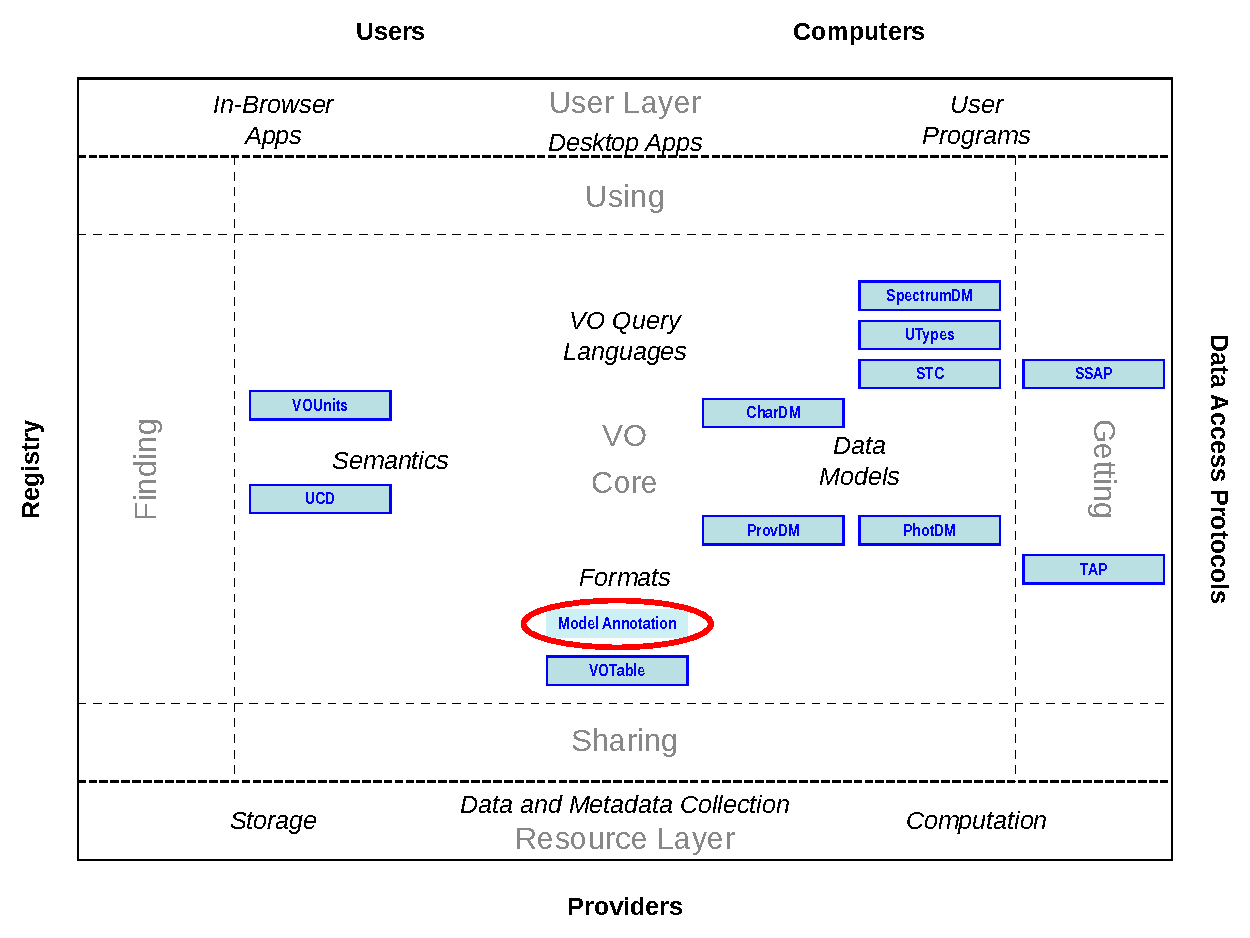
\includegraphics[width=0.9\textwidth]{role_diagram.pdf}
\caption{Architecture diagram for this document}
\label{fig:archdiag}
\end{figure}

Fig.~\ref{fig:archdiag} shows the role this document plays within
the IVOA architecture \citep{2010ivoa.rept.1123A}.


\pagebreak
\section{Use Cases and Requirements}

\subsection{Use Cases}


The mapping syntax allows to map data on any model compliant with VODML. 
Annotation blocks denote the model structure and contain references to the appropriate
FIELDs and PARAMs. Model-aware clients can build model instances just by reading the annotation
block and by resolving the references to set the model leaf values. 

Such a mechanism allows the client to get a better understanding of the data complexity.
The annotation block is designed in a way that clients are not forced to choose between a regular data processing and a full object approach.
There are intermediate levels of use that correspond to concrete use cases that are addressed by this standard.



\begin{itemize}
  \item Coordinate or calibration Systems: The recent modelling efforts (Coords and PhotDM) provide a very accurate description of coordinate frames or photometric systems that need to be serialised in VOTables:
  \begin{itemize}
    \item Clients often need to get an accurate representation of the coordinate systems to make the best of many datasets  
    \item Data sets can contain multiple quantities expressed in the same coordinate system (corrected position vs raw position) or 
             quantities of the same nature but expressed in different systems (sky coordinates in ICRS vs Gal). %NFB different COOSYS can be set in reference from the FIELDS. But COOSYS is limited. I think it's the real argument.
  \end{itemize} 
  
  \item Quantities made with "multiple components (data columns) that must be gathered by the client to be properly used:
  \begin{itemize}
    \item value-error associations
    \item error quantities split in several columns (covariance matrices). 
    \item quantities with quality flags
    \item positions with proper motions and/or parallax to compute error ellipses or positions at a given epoch
  \end{itemize} 

  \item The above cases relate to the processing of individual datasets; 
  
  the model annotations become even more important for cases where a good level of interoperability is required to match different datasets. 
           This can be achieved by giving  common data structures for all quantities of interest. This is the purpose of e.g. Measure model which proposes classes for 
           most of the physical quantities and can be rendered by the mapping syntax. Measure classes are not meant to be used as standalone elements but as parts of host models (e.g. CubeDM, Mango);
           however clients keep free to either process those host models as a whole or to chase individual components.
    \begin{itemize}
      \item Cross matching VOTables having all the same accurate description of e.g. the sky position is easier. %(FB : what does that mean "accurate description" ? Space Frame ? unit ? ) 
               This also improves the reliability of the process since the engine does not need to infer information that is not in the FIELD meta-data.
      \item Building SEDs from datasets that have the same accurate photometry representation is straightforward.
   \end{itemize}          

  \item In more advanced cases, we need to be able to extract complete model instances from VOTables.
    \begin{itemize}
      \item Extracting  TimeSeries instances to feed a software built upon classes generated from that model.
      \item Building model instances that can be serialised in another format (e.g. json) in order to be shared in another context than the VOTable processing (e.g. via SAMP).
   \end{itemize}         
    
   \item The mapping syntax can be used to annotate static science products such as e.g. time-series. It can also be used to annotate on the fly TAP responses.
   As shown by (ref- Mireille ADASS) this process is not always possible because the model compliance of the searched data strongly depends on the executed query (missing searched columns, joins, data aggregation ...). 
   However, clients connecting TAP services registered as delivering annotated data would expect to get annotation blocks in query responses even if the annotation process is not possible. 
   This feature must be supported by the proposed syntax.
    
\end{itemize} 




\subsection{Requirements}
\begin {itemize}
  \item Shy annotation: model annotations come in a workflow which has been working very well for years, this is why the first requirement is to keep any existing stakeholder unbroken.
  \begin {itemize}
    \item Annotation must not alter the VOTable content.
    \item Annotation blocks must be located in a way that it can easily be skipped by model-unaware clients.
    \item The vocabulary in the annotation name-space must not overlap with the VOTable elements (names or attributes)    
    \item The annotation syntax must be able to inform the client about the status of the annotation process.
  \end {itemize}
  
  \item Schema and validation:
  \begin {itemize}
    \item The annotation schema must be independent from the VOTable schema.
    \item The evolution of the annotation schema must not impact the VOTable schema.
    \item The evolution of the VOTable schema must not impact the annotation schema.
    \item The annotation syntax must be validated using the usual tools, i.e. without using specific compilers.
    \item Validators are not meant to check whether references can be resolved. Clients are in charge of handling such inconsistencies.
  \end {itemize}
  
  \item Model agnostic behavior:
  \begin {itemize}
    \item The annotation syntax must be able to map data on any \texttt{VODML} compliant model
    \item The annotation syntax must allow clients to use their own strategy to consume mapped data:
      \begin {itemize}
        \item just ignore it
        \item just pick some elements of interest 
        \item just pick model meta-data and process the stream of data rows as usual
        \item pick whole model instances
      \end {itemize}
  \end {itemize}
  
  \item On the fly annotation status:
      \begin {itemize} 
          \item Clients connecting TAP services registered as delivering annotated data must get VOTable with annotation blocks in any cases. 
          \item Clients must be informed on the status of the annotation process.          
       \end {itemize}

\end {itemize}



% use XML formatting for listings
\lstset{language=XML}

\pagebreak
\section{Relation to VOTable}

The data model annotation will reside within the scope of a VOTABLE V1.1+ (TBCheck)

\noindent \textbf{Location}

The mapping block:
\begin{itemize}
\item MUST be contained in a VOTable RESOURCE with \texttt{type="meta"}. This extra feature is consistent with VOTable xml schema RESOURCE type definition and doesn't require any modification in the xml schema.
\item which MUST be the first child of a RESOURCE with \texttt{type="results"}.
\item there MUST be no more than one mapping block per 'results' RESOURCE.
\end{itemize}

The scope of the mapping block is the whole content of the 'results' RESOURCE. \newline

\noindent \textbf{Namespace}

The \texttt{dm-mapping} name space isolates VOTable elements from mapping elements, and MUST be defined on the mapping block. \newline

\begin{lstlisting}[frame=single,caption={Mapping block in a VOTable},style=XML,basicstyle=\tiny]
<VOTABLE xmlns="http://www.ivoa.net/xml/VOTable/v1.3" 
         xmlns:xsi="http://www.w3.org/2001/XMLSchema-instance" version="1.3">
  <RESOURCE type="results">
    <RESOURCE type="meta">
      <dm-mapping:VODML xmlns:dm-mapping="http://www.ivoa.net/xml/merged-syntax">
        ...
      </dm-mapping:VODML>
    </RESOURCE>
    <TABLE name="myDataTable">
      ....
    </TABLE>
  </RESOURCE>
</VOTABLE>
\end{lstlisting}


\pagebreak
\section{Syntax}

The syntax has been designed to use as less XML elements as possible and to rely on XML attributes to setup the element behavior in a particular context.
As shown in \ref{tbl:syntax-ele} the mapping elements  can be grouped in 3 different scopes. There are only 3 elements for the models structure itself. We assume that any data hierarchy  can be represented a combination of collections (COLLECTION), tuples (INSTANCE) and simple values (ATTRIBUTE). The others elements are either set the mapping block structure or to connect data to each other.

\begin{table}[!htbp]
\small
\centering
\begin{tabulary}{\linewidth}{|c|J|}       
       \hline 
            \textbf{Scope} & 
            \textbf {Elements}\\
       \hline         
       \hline  
             Data modeling tags & 
             ATTRIBUTE INSTANCE COLLECTION \\
       \hline  
             Mapping block structre & 
             VODML MODEL REPORT TEMPLATES GLOBALS \\
       \hline  
             Data references and identification & 
             REFERENCE JOIN  FOREIGN\_KEY PRIMARY\_KEY WHERE\\
       \hline
     \end{tabulary}
     \caption{Mapping elements grouped by scopes} 
     \label{tbl:syntax-ele}
\end{table}


As shown in \ref{tbl:syntax-att} and following the VODML pattern, any model node is characterized by a role (@dmrole) and a type (@dmtype). All of the others attributes are used to bind data with either VOtable elements or others mapping elements.
 
\begin{table}[!htbp]
\small
\centering
\begin{tabulary}{\linewidth}{|c|J|}       
       \hline 
            \textbf{Scope} & 
            \textbf {Attributes}\\
       \hline         
       \hline  
             Model related & 
             @name @uri \\
       \hline  
             Modeled node related & 
             @dmrole @dmtype \\
       \hline  
             Related to attribute values & 
             @value @unit @arrayindex \\
       \hline  
             Related to VOTable elements & 
             @tableref @ref\\
       \hline  
             Mapping element identification& 
             @dmref @dmid @url @dmid @sourceref @primarykey @foreignkey\\
       \hline
     \end{tabulary}
     \caption{Attributes of mapping elements grouped by scopes} 
     \label{tbl:syntax-att}
 \end{table}
 
 


  \begin{figure}[h]
    \begin{center}
      \includegraphics[width=\textwidth]{merged-syntax-summary.png}
      \caption{Annotation Syntax Summary}
      \label{fig:summary}
    \end{center}
  \end{figure}



\pagebreak
\subsection{VODML}
The \texttt{VODML} element is the top level container for the mapping elements for a single VOTable RESOURCE.
When the mapping \texttt{REPORT} is set to KO, the others  VOTable children are optional.

\begin{lstlisting}[frame=single,caption={Example \texttt{VODML} mapping block},style=XML,basicstyle=\tiny]
<dm-mapping:VODML>
  <dm-mapping:REPORT status="OK"/>
  <dm-mapping:MODEL>  ...  </dm-mapping:MODEL>
  <dm-mapping:GLOBALS>  ...  </dm-mapping:GLOBALS>
  <dm-mapping:TEMPLATES>  ...  </dm-mapping:TEMPLATES>
   ...
</dm-mapping:VODML>
\end{lstlisting}

\begin{table}[!htbp]
  \small
  \centering
  \begin{tabulary}{\linewidth}{|c |c |c|}
    \hline 
        \textbf{Element} &
        \textbf{Position} &
        \textbf{Occurs}\\
    \hline
    \hline  
      \texttt{REPORT} &           
      1 &           
      0-1\\
    \hline  
      \texttt{MODEL} &           
      2 &           
      0-*\\
    \hline    
      \texttt{GLOBALS} &           
      3 &           
      0-*\\
    \hline  
      \texttt{TEMPLATES} &           
      4 &           
      0-*\\
    \hline 
  \end{tabulary}
    \caption{Allowed children for \texttt{VODML}} 
    \label{tbl:vodml-children}
\end{table}



\FloatBarrier

\subsection{REPORT}
Services providing annotated responses must use the \texttt{REPORT}  element to tell the client whether the annotation process succeeded or not.

\begin{itemize}
\item \texttt{REPORT} is not mandatory.
\item It must be the first \texttt{VODML} child if present.
\end{itemize}



\begin{lstlisting}[frame=single,caption={Example of a \texttt{REPORT} element},style=XML,basicstyle=\tiny]
<dm-mapping:VODML
	xmlns:dm-mapping="http://www.ivoa.net/xml/merged-syntax">
	
	<dm-mapping:REPORT status="KO">
	    The annotation process failed
	</dm-mapping:REPORT>

	<dm-mapping:MODEL name="model" url="http://aaaaaa" />
	<dm-mapping:MODEL name="model" />
	
</dm-mapping:VODML>
\end{lstlisting}

\begin{table}[!htbp]
  \small
  \centering
  \begin{tabulary}{\linewidth}{|c|J|}       
    \hline 
         \textbf{Attribute} & 
         \textbf {Role}\\
    \hline
    \hline  
         @status  & 
        Status of the annotation process; must be either \texttt{OK} or \texttt{KO} \\
    \hline 
  \end{tabulary}
  \caption{\texttt{REPORT} attributes} 
  \label{tbl:report-att}
\end{table}


\FloatBarrier
 
\subsection{MODEL}
A VOTable can provide serializations for an arbitrary number of data model
types. In order to declare which models are represented in the file, data
providers must declare them through the \texttt{MODEL} elements.
Only models that are used in the file must be declared. A model is
used if at least one element in the mapping block refer to it. In other terms, only models that define vodml-ids used in the
annotation must be declared.

\begin{lstlisting}[frame=single,caption={Example \texttt{MODEL} mapping block},style=XML,basicstyle=\tiny]
<dm-mapping:VODML>
  <dm-mapping:MODEL name="sample-ext"
                     url="https://www.myorg.net/models/SampleExt-v1.0.vo-dml.xml" />
  <dm-mapping:MODEL name="sample" url="https://www.ivoa.net/xml/DNE/Sample-v1.0.vo-dml.xml" />
  <dm-mapping:MODEL name="ivoa"   url="https://www.ivoa.net/xml/VODML/IVOA-v1.vo-dml.xml" />
</dm-mapping:VODML>
\end{lstlisting}

\begin{table}[!htbp]
  \small
  \centering
  \begin{tabulary}{\linewidth}{|c|J|}       
    \hline 
         \textbf{Attribute} & 
         \textbf {Role}\\
    \hline
    \hline  
         \texttt{@name}  & 
         Name of the mapped model as declared in the \texttt{VODML} XML model serialization.  This attribute MUST not be empty and forms the prefix used in  \texttt{@dmrole} dmtype tags of elements from that model.  \\
    \hline 
         \texttt{@url} & 
         URL to the vo-dml serialization of the model. If present, this attribute MUST not be empty.\\
    \hline 
  \end{tabulary}
  \caption{\texttt{MODEL} attributes} 
  \label{tbl:model-att}
\end{table}


\begin{table}[!htbp]
  \small
  \centering
  \begin{tabulary}{\linewidth}{|c |c |J|}
    \hline 
        \textbf{@name} &
        \textbf{@url} &
        \textbf{Pattern}\\
    \hline      \hline  
        MAND &           
        OPT &           
        Unique attribute pattern supported by \texttt{MODEL}\\
    \hline 
  \end{tabulary}
  \caption{Valid attribute patterns for  \texttt{MODEL}} 
  \label{tbl:model-pattern}
\end{table}

\FloatBarrier

\subsection{GLOBALS}
The \texttt{GLOBALS} block holds singular data model instances, and is not associated 
with a VOTable \texttt{TABLE}.

The contained instances have a global scope, and may be
referenced by other instances anywhere in the mapping block.  \texttt{INSTANCE} attributes
within the \texttt{GLOBALS} scope may only refer to VOTable \texttt{PARAMS} or contain
explicit values, they MUST NOT refer to VOTable \texttt{FIELDS}.  Note: This rule is not enforced
via the XSD schema which is restricted to the mapping block only.

Related instances may be grouped within a \texttt{COLLECTION} block to enable selection
via the ORM elements provided in this syntax.  See \texttt{COLLECTION} for more details.

\begin{lstlisting}[frame=single,caption={Example \texttt{GLOBALS} block},style=XML,basicstyle=\tiny]
<dm-mapping:VODML>
  <dm-mapping:MODEL name="sample" url="https://www.ivoa.net/xml/DNE/Sample-v1.0.vo-dml.xml" />
  <dm-mapping:MODEL name="ivoa"   url="https://www.ivoa.net/xml \texttt{VODML} IVOA-v1.vo-dml.xml" />
  <dm-mapping:GLOBALS>
    <!-- a collection of coordinate systems -->
    <dm-mapping:COLLECTION dmid="\_CoordinateSystems" >
      <dm-mapping:INSTANCE dmid="\_timesys" dmtype="sample:TimeSys">
         ...
      </dm-mapping:INSTANCE>
      <dm-mapping:INSTANCE dmid="\_spacesys" dmtype="sample:SpaceSys">
         ...
      </dm-mapping:INSTANCE>
    </dm-mapping:COLLECTION>

    <!-- a singular, stand-alone instance -->
    <dm-mapping:INSTANCE dmtype="sample:Thing">
      <dm-mapping:ATTRIBUTE dmrole="sample:Thing.name" dmtype="ivoa:string" value="MyThing"/>
      <dm-mapping:ATTRIBUTE dmrole="sample:Thing.date" dmtype="ivoa:string" ref="\_date"/>
      ...
    </dm-mapping:INSTANCE>
  </dm-mapping:GLOBALS>
</dm-mapping:VODML>
\end{lstlisting}


\begin{table}[!htbp]
  \small
  \centering
  \begin{tabulary}{\linewidth}{|c |c |c|}
    \hline 
        \textbf{Element} &
        \textbf{Position} &
        \textbf{Occurs}\\
    \hline
    \hline
        \texttt{INSTANCE} &
        Any &
        0-*\\
    \hline
        \texttt{COLLECTION} &
        Any &
        0-*\\
    \hline
  \end{tabulary}
  \caption{Allowed children for \texttt{GLOBALS}} 
  \label{tbl:globals-children}
 \end{table}

\FloatBarrier

\subsection{TEMPLATES}
The \texttt{TEMPLATES} block defines a template for deriving multiple data model instances,
one for each row of the associated VOTable \texttt{TABLE}.  A subset of the associated
\texttt{TABLE} rows may be selected using the \texttt{WHERE} syntax element.

\begin{lstlisting}[frame=single,caption={Example \texttt{TEMPLATES} block},style=XML,basicstyle=\tiny]
<dm-mapping:VODML>
  <dm-mapping:MODEL name="sample" url="https://www.ivoa.net/xml/DNE/Sample-v1.0.vo-dml.xml" />
  <dm-mapping:MODEL name="ivoa"   url="https://www.ivoa.net/xml \texttt{VODML} IVOA-v1.vo-dml.xml" />
  <dm-mapping:TEMPLATES tableref='Results'>
    <!-- instance template -->
    <dm-mapping:INSTANCE dmtype="sample:Thing">
      <dm-mapping:ATTRIBUTE dmrole="sample:Thing.name" dmtype="ivoa:string" ref="\_field1"/>
      <dm-mapping:ATTRIBUTE dmrole="sample:Thing.date" dmtype="ivoa:string" ref="\_field2"/>
      ...
    </dm-mapping:INSTANCE>
  </dm-mapping:TEMPLATES>
</dm-mapping:VODML>
\end{lstlisting}

\begin{table}[!htbp]
  \small
  \centering
  \begin{tabulary}{\linewidth}{|c|J|}
    \hline 
         \textbf{Attribute} & 
         \textbf {Role}\\
    \hline
    \hline  
         \texttt{@tableref} & 
         ID of the mapped VOTable \texttt{TABLE}.\\
    \hline 
  \end{tabulary}
  \caption{\texttt{TEMPLATES} attributes} 
  \label{tbl:templates-att}
\end{table}

\begin{table}[!htbp]
  \small
  \centering
  \begin{tabulary}{\linewidth}{|c|J|}
    \hline 
        \textbf{@tableref} &
        \textbf{Pattern}\\
    \hline
    \hline  
        OPT &           
        If \texttt{@tableref} is not present, \texttt{TEMPLATES} maps the first \texttt{TABLE} of the \texttt{RESOURCE}\\
    \hline 
  \end{tabulary}
  \caption{Valid attribute patterns for  \texttt{TEMPLATES}} 
  \label{tbl:templates-pattern}
 \end{table}

\begin{table}[!htbp]
  \small
  \centering
  \begin{tabulary}{\linewidth}{|c |c |c|J|}
    \hline 
        \textbf{Element} &
        \textbf{Position} &
        \textbf{Occurs} &
        \\
    \hline
    \hline  
        \texttt{WHERE}  &        
        1 &           
        0-* &
        The mapping applies to rows matching the \texttt{WHERE} condition only\\
    \hline    
        \texttt{INSTANCE} &           
        2 &           
        0-* &
        Mapped instance templates\\
    \hline 
  \end{tabulary}
  \caption{Allowed children for \texttt{TEMPLATES}} 
  \label{tbl:templates-children}
\end{table}

\FloatBarrier

\subsection{COLLECTION}
    \texttt{COLLECTION} is a container element.  It is used in different contexts, each allowing a limited subset of elements for its content. 
    
    \texttt{COLLECTION} can be populated either by a static list of items  \texttt{INSTANCE}  \texttt{ATTRIBUTE} ..) or by joining to another \texttt{COLLECTION} (using the \texttt{JOIN} element). Both  modes cannot coexist.
    
    \begin{enumerate}
    \item{As child of INSTANCE}
      
      The \texttt{COLLECTION} serves as a container for elements with multiplicity $>$ 1.\\
      Examples of usage in this context would be:
      \begin{itemize}
        \item an array attribute
        \item a reference relation with multiplicity $>$ 1
        \item a composition relation with multiplicity $>$ 1
      \end{itemize}
      
    \item{As child of GLOBALS}
          
      The \texttt{COLLECTION} serves as a proxy for TABLE, grouping common \texttt{INSTANCE}  for selection by PRIMARY \texttt{FOREIGN\_KEY} 
      Examples of usage in this context would be:
      \begin{itemize}
        \item a set of photometry filters, which apply to various rows of a photometric data table, based on the value of the 'band' column.
        \item a set of Dataset metadata instances, which apply to various rows of a photometric data table, based on the value of the 'id' column.
      \end{itemize}
          
    \item{As child of COLLECTION}
	The collection contains a matrix of  atomic values
        
    \end{enumerate}
   
\begin{lstlisting}[frame=single,caption={Example of \texttt{COLLECTION} child of INSTANCE},style=XML,basicstyle=\tiny]
<dm-mapping:INSTANCE dmtype="model:Thing">
    <dm-mapping:COLLECTION dmrole="model:Thing.elems">
        <dm-mapping:ATTRIBUTE dmtype="model:Foo" value="100" />
        <dm-mapping:ATTRIBUTE dmtype="model:Foo" value="110" />
    </dm-mapping:COLLECTION>
</dm-mapping:INSTANCE>
\end{lstlisting}   

\begin{lstlisting}[frame=single,caption={Example of \texttt{COLLECTION} child of GLOBALS},style=XML,basicstyle=\tiny]
<dm-mapping:GLOBALS>
    <dm-mapping:COLLECTION dmid="_filters" >
        <dm-mapping:INSTANCE dmtype="model:PhotometryFilter" >
            <dm-mapping:PRIMARY_KEY dmtype="ivoa:string" value="RP"/>
            <dm-mapping:ATTRIBUTE dmrole="model:PhotometryFilter.name" dmtype="ivoa:string"
                                    value="GAIA/GAIA2r.Grp"/>
        </dm-mapping:INSTANCE>
        <dm-mapping:INSTANCE dmtype="model:PhotometryFilter" >
            <dm-mapping:PRIMARY_KEY dmtype="ivoa:string" value="BP"/>
            <dm-mapping:ATTRIBUTE dmrole="model:PhotometryFilter.name" dmtype="ivoa:string"
                                    value="GAIA/GAIA2r.Gbp"/>
        </dm-mapping:INSTANCE>
    </dm-mapping:COLLECTION>
<dm-mapping:GLOBALS>
\end{lstlisting}   

\begin{lstlisting}[frame=single,caption={Example of \texttt{COLLECTION} populated with a JOIN},style=XML,basicstyle=\tiny]
<dm-mapping:GLOBALS>
    <dm-mapping:COLLECTION dmrole="_joined_dataj">
        <dm-mapping:JOIN tableref="_someTemplates" dmref="_extInst"/>
    </dm-mapping:COLLECTION>
<dm-mapping:GLOBALS>
\end{lstlisting}   


\begin{table}[!htbp]
  \small
  \centering
  \begin{tabulary}{\linewidth}{|c|J|}       
    \hline 
         \textbf{Attribute} & 
         \textbf {Role}\\
    \hline
    \hline  
         \texttt{@dmid} & 
         Element datamodel id, MUST be unique within the document.\\
    \hline 
         \texttt{@dmrole} & 
         Role of the \texttt{COLLECTION} in the data model. \\
    \hline 
  \end{tabulary}
  \caption{\texttt{COLLECTION} attributes} 
  \label{tbl:collection-att}
 \end{table}

\begin{table}[!htbp]
  \small
  \centering
  \begin{tabulary}{\linewidth}{|c|c|c|J|}
    \hline 
      \textbf{Context} &
      \textbf{@ID} &
      \textbf{@dmrole} &
      \textbf{Pattern}\\
    \hline      \hline  
      1 &
      OPT & 
      MAND & 
      The element maps a collection playing a role in a modeled \texttt{INSTANCE}.  \texttt{@dmrole} MUST  be not empty.  If present, \texttt{@dmid} MUST  be not empty. \\
    \hline   
      2 &
      MAND & 
      NO & 
      The collection, has no role. MUST have non-empty dmid to reference for ORM selection of contained \texttt{INSTANCE}. This occurs when e.g. the \texttt{COLLECTION} is a \texttt{GLOBALS} child.\\
    \hline 
  \end{tabulary}
  \caption{Valid attribute patterns for \texttt{COLLECTION}} 
  \label{tbl:collection-pattern}
 \end{table}


\begin{table}[!htbp]
  \small
  \centering
  \begin{tabulary}{\linewidth}{|c|c|c|J|}
    \hline 
      \multicolumn{4}{|l|}{\textbf{Context: Child of INSTANCE}} \\
    \hline 
      \textbf{Element} &
      \textbf{Position} &
      \textbf{Occurs}  \\
    \hline
    \hline  
        \texttt{ATTRIBUTE} & 
        Only & 
        0-* & 
        Collection of attributes.\\
    \hline    
        \texttt{REFERENCE} & 
        Only & 
        0-* & 
        Collection of references.\\
    \hline    
        \texttt{INSTANCE} & 
        Any & 
        0-* & 
        Collection of instances.\\
    \hline    
        \texttt{JOIN} & 
        Any & 
        0-1 & 
        Collection populated with a set of joined instances. No other child is supported in this case\\
    \hline    
        \texttt{COLLECTION} & 
        Only & 
        0-* & 
        Collection of collections.\\
    \hline    
    \hline 
      \multicolumn{4}{|l|}{\textbf{Context: Child of GLOBALS}} \\
    \hline 
      \textbf{Element} &
      \textbf{Position} &
      \textbf{Occurs} &  \\
    \hline
    \hline    
        \texttt{INSTANCE} & 
        Only & 
        0-* & 
        Collection of related instances.\\
    \hline    
        \texttt{REFERENCE} & 
        Only & 
        0-* & 
        Collection of related references.\\
    \hline 
  \end{tabulary}
     \caption{Allowed children for \texttt{COLLECTION}} 
     \label{tbl:collection-chilren}
 \end{table}

\FloatBarrier

\subsection{INSTANCE}
The \texttt{INSTANCE} element defines a complex ObjectType or DataType.
It may be a child of several other elements, and the requirements on
the content (especially dmid and dmrole), may differ depending on
the usage:


\begin{enumerate}
\item Child of \texttt{GLOBALS}

   In this case the \texttt{INSTANCE} is a single stand-alone instance which
   may or may not be referenced by other \texttt{INSTANCE} . This pattern is typically used for 
   shared object e.g. space frames, or for head object of science product models e.g. Time Series
  \begin{itemize}
     \item May have dmid attribute, as possible target of \texttt{REFERENCE} ref
     \item must have no  \texttt{dmrole} attribute or an empty one
  \end{itemize}  
     
\item Child of \texttt{TEMPLATES} 
  In this case, the \texttt{INSTANCE} is a template for instances which
  are generated once per row of the associated table.  
  \begin{itemize}
     \item may have dmid attribute, as target of \texttt{JOIN} dmref
     \item must have no  \texttt{dmrole} attribute or an empty one
  \end{itemize}  

\item Child of \texttt{COLLECTION} 
  There are 2 uses for this pattern.  
  \begin{itemize}
     \item each member \texttt{INSTANCE} is a target for selection using
           the PRIMARY \texttt{FOREIGN\_KEY} elements. This pattern is only 
           allowed within the \texttt{GLOBALS} environment. In this case:             
           \begin{itemize}
             \item must contain at least one \texttt{PRIMARY\_KEY} sub-element
             \item may have a dmid attribute, as possible target of \texttt{REFERENCE}              \item must have no  dmrole attribute or an empty one. \texttt{VODML} does set roles to particular collection items
           \end{itemize}

     \item Elements \texttt{INSTANCE} are collection cells with multiplicity > 1
          Each one :             
           \begin{itemize}
             \item must have no dmrole attribute or an empty one
           \end{itemize}
  \end{itemize}  
    
\item Child of \texttt{INSTANCE}  
     In this case, each \texttt{INSTANCE} represents 
     a complex ObjectType or DataType playing a role in the parent \texttt{INSTANCE}      
     \begin{itemize}
        \item may have dmid attribute
        \item must have non-empty dmrole attribute
     \end{itemize}
           
\item any \texttt{INSTANCE}      
   \begin{itemize}
        \item if dmid attribute is present, it must not be empty
        \item must have non-empty dmtype attribute
    \end{itemize}
\end{enumerate}  
    
   
\begin{lstlisting}[frame=single,caption={Example of \texttt{INSTANCE} child of GLOBALS},style=XML,basicstyle=\tiny]
<dm-mapping:INSTANCE dmid="SpaceFrame_ICRS" dmtype="coords:SpaceFrame">
	<dm-mapping:INSTANCE dmrole="coords:SpaceFrame.refPosition"
                                 dmtype="coords:StdRefLocation">
		<dm-mapping:ATTRIBUTE dmrole="coords:StdRefLocation.position" 
		                          dmtype="ivoa:string"  value="NoSet" />
	</dm-mapping:INSTANCE>
	<dm-mapping:ATTRIBUTE dmrole="coords:SpaceFrame.spaceRefFrame" 
	                          dmtype="ivoa:string" value="ICRS" />
	<dm-mapping:ATTRIBUTE dmrole="coords:SpaceFrame.equinox" 
	                          dmtype="coords:Epoch"	value="2015" />
</dm-mapping:INSTANCE>
\end{lstlisting}   
   

\begin{table}[!htbp]
\small
\centering
\begin{tabulary}{\linewidth}{|c|J|}       
       \hline 
            \textbf{Attribute} & 
            \textbf {Role}\\
       \hline         \hline  
            \texttt{@dmid} & 
            Element dmid, MUST be unique within the mapping block  \\
        \hline 
            \texttt{@dmrole} & 
            \texttt{INSTANCE} role played in the DM \\
        \hline 
            \texttt{@dmtype} & 
            Class name in a model context\\
        \hline 
     \end{tabulary}
     \caption{\texttt{INSTANCE} attributes} 
     \label{tbl:instance-att}
 \end{table}   
 


 
\begin{table}[!htbp]
\small
\centering
\begin{tabulary}{\linewidth}{|c |c |c|J|}
    \hline 
        \textbf{Element} &
        \textbf{Position} &
        \textbf{Occurs} &
        \\
    \hline      \hline  
        \texttt{PRIMARY\_KEY}  &        
        First &           
        0-* &
        Primary key to be used to in a \texttt{JOIN} context.\\
    \hline    
        \texttt{REFERENCE}  &        
        Any &           
        0-* &
         Object attribute as a reference to either another \texttt{INSTANCE} or a \texttt{COLLECTION} \\
    \hline    
        \texttt{INSTANCE} &           
        Any &           
        0-* &
         Object attribute as a class instance. \\
    \hline    
        \texttt{ATTRIBUTE} &           
        Any &           
        0-* &
       Object attribute as a simple attribute. \\
    \hline    
        \texttt{COLLECTION} &           
        Any &           
        0-* &
         Object attribute  as a collection.\\
    \hline 
\end{tabulary}
     \caption{Allowed children for \texttt{INSTANCE}} 
     \label{tbl:instance-chilren}
\end{table}
 
\begin{table}[!htbp]
\small
\centering
\begin{tabulary}{\linewidth}{|c|c|c|J|}
    \hline 
        \textbf{@dmid} &
        \textbf{@dmrole} &
        \textbf{@dmtype} &
        \textbf{Pattern}\\
    \hline      \hline  
        OPT &           
        NO or EMPTY&           
        MAND &           
        MUST be applied when the  \texttt{INSTANCE} is child of \texttt{GLOBALS} or \texttt{TEMPLATES}. The element has no role because it is not embedded in a model component. It must be referable by a \texttt{REFERENCE}  \\
    \hline   
        OPT &           
        MAND &           
        MAND &           
        MUST be applied in any other location. It may be referable a \texttt{REFERENCE} . \\
   \hline 
\end{tabulary}
     \caption{Valid attribute patterns for  \texttt{INSTANCE}} 
     \label{tbl:instance-pattern}
 \end{table}       
\newpage

 

\FloatBarrier

\subsection{ATTRIBUTE}

The \texttt{ATTRIBUTE} element defines either a class attribute or a collection item, both set with atomic values.
The requirements on
the content (especially ref and  \texttt{@dmrole}, may differ depending on
the usage:


\begin{enumerate}
\item Descendant of \texttt{GLOBALS}

In this case, the \texttt{ATTRIBUTE} must be specified by:
  \begin{itemize} 
      \item \texttt{@ref} - reference to a VOTable \texttt{PARAM}, 
      (not a VOTable \texttt{FIELD})
      \item \texttt{@value} - a literal
      \item  if both are provided; \texttt{@value} serves as the default 
      if the reference cannot be resolved
  \end{itemize}  

  
\item Descendant of \texttt{TEMPLATES} 

In this case, the \texttt{ATTRIBUTE} must be specified by:
  \begin{itemize} 
      \item \texttt{@ref} - reference to a VOTable \texttt{PARAM} 
      or \texttt{FIELD}
      \item \texttt{@value} - a literal
      \item if both are provided, \texttt{@value} serves as the default if 
      the reference cannot be resolved
  \end{itemize}  

\item Child of \texttt{COLLECTION} :
    The \texttt{ATTRIBUTE} can be seen as a vector coordinate, 
    it must have  no \texttt{@dmrole} xml attribute or an empty one
    
\item Child of \texttt{INSTANCE} :
    The \texttt{ATTRIBUTE} can be seen as a class attribute, 
    it must have a \texttt{@dmrole} xml attribute
           
\item Any case :     
    The \texttt{ATTRIBUTE} must always have a non empty \texttt{@dmtype} xml attribute.
\end{enumerate}  
    
    
\begin{lstlisting}[frame=single,caption={ATTRIBUTE examples},style=XML,basicstyle=\tiny]
<dm-mapping:INSTANCE dmtype="model:Thing">
    <dm-mapping:ATTRIBUTE dmrole="model:Thing.f" dmtype="model.Alpha" value="xyz"/>		
    <dm-mapping:INSTANCE dmrole="model:Thing.pos" dmtype="adhoc:Position">
        <dm-mapping:ATTRIBUTE dmrole="adhoc:Position.longitude" dmtype="ivoa:real" 
                        ref="_eqpos" arrayindex="0"/>
        <dm-mapping:ATTRIBUTE dmrole="adhoc:Position.latitude" dmtype="ivoa:real" 
                        ref="_eqpos" arrayindex="1"/>
    </dm-mapping:INSTANCE>
</dm-mapping:INSTANCE>
\end{lstlisting}  


\begin{table}[!htbp]
\small
\centering
\begin{tabulary}{\linewidth}{|c|J|}       
       \hline 
            \textbf{Attribute} & 
            \textbf {Role}\\
       \hline         \hline  
            \texttt{@dmrole} & 
            Role of the attribute in the DM\\
        \hline 
            \texttt{@dmtype} & 
            Type of the attribute in the DM\\
        \hline 
            \texttt{@ref} & 
            Reference of the \texttt{FIELD} that has to be used to set the 
            \texttt{ATTRIBUTE} value.\\
        \hline 
            \texttt{@value}  &
            Default \texttt{ATTRIBUTE} value. This value is taken if there is no 
            \texttt{@ref} attribue or if \texttt{@ref} cannot be resolved.\\
        \hline 
            \texttt{@unit} & 
            \texttt{ATTRIBUTE} unit. This is the unit in which the native value must be 
            converted to be compliant with the model. This attribute is always optional.\\
        \hline 
            \texttt{@arrayindex} & 
            Index of the native value to be taken to set the \texttt{ATTRIBUTE}. 
            The value must be >= 0.
            Must be ignored if the native value is a single value. 
            An error must be risen if \texttt{@arrayindex} is out of range.
            This attribute is always optional.\\
        \hline 
     \end{tabulary}
     \caption{\texttt{ATTRIBUTE} attributes} 
     \label{tbl:attribute-att}
 \end{table}

\begin{table}[!htbp]
\small
\centering
\begin{tabulary}{\linewidth}{|c|c|c|c|c|J|}
    \hline 
        \textbf{@dmrole} &
        \textbf{@dmtype} &
        \textbf{@ref} &
        \textbf{@value} &
        \textbf{@arrayindex} &
        \textbf{Pattern}\\
    \hline     
    \hline  
        MAND &           
        MAND &           
        OPT &           
        OPT &           
        OPT &   
        1 \\
    \hline   
        MAND &           
        MAND &           
        NO &           
        MAND &           
        OPT &   
        2\\
    \hline  
        NO &           
        MAND &           
        OPT &           
        OPT &           
        OPT &   
        3 \\
   \hline 
\end{tabulary}
     \caption{Valid attribute patterns for \texttt{ATTRIBUTE}. (1) Valid in a \texttt{TEMPLATES} context.        
        The \texttt{ATTRIBUTE} value must be set with the value of the element referenced by \texttt{@ref} 
       If the \texttt{@ref} can not be resolved and \texttt{@value} is present, \texttt{@value} must be taken. Either \texttt{@ref} or \texttt{@value} must be present or both (2) This pattern 
        is valid in any context.  (3) is valid in the context of a \texttt{COLLECTION} item.    
        The \texttt{ATTRIBUTE} value must be set with \texttt{@value}         as \texttt{ATTRIBUTE} value} 
     \label{tbl:attribute-pattern}
 \end{table}

\FloatBarrier

\subsection{REFERENCE}
INSTANCE reference that can be used with the same patterns as for \texttt{INSTANCE} .
There are different uses for the \texttt{REFERENCE} 

\begin{itemize}
    \item Static reference: the element has a \texttt{@dmref} attribute that matches the \texttt{@dmid} attribute of the referenced \texttt{INSTANCE} 
    \item Dynamic reference: The element has a \texttt{@sourceref} attribute identifying  the table where to fetch the referenced column. 
    
             In this case, \texttt{REFERENCE} must be located in a \texttt{TEMPLATES} and it must have one or more \texttt{FOREIGN\_KEY} children. 
             If the referenced table contains several \texttt{INSTANCE} with a \texttt{PRIMARY\_KEY}  the first one must be taken by default.
\end{itemize}

\begin{lstlisting}[frame=single,caption={Simple \texttt{REFERENCE}, to be replaced with the \texttt{INSTANCE} having \texttt{@dmid} \_target1 },style=XML,basicstyle=\tiny]
<dm-mapping:REFERENCE dmrole="_role" dmref="_target1" />
\end{lstlisting}

\begin{lstlisting}[frame=single,caption={Dynamic \texttt{REFERENCE}, to be replaced with the \texttt{INSTANCE} of the table of collection \_target1 and having a \texttt{PRIMARY\_KEY} matching the value of column  \_col1. This pattern is valid in the context of a TEMPLATES},style=XML,basicstyle=\tiny]
<dm-mapping:REFERENCE dmrole="_role" sourceref="_target1">
    <dm-mapping:FOREIGN_KEY ref="_col1" />
</dm-mapping:REFERENCE>
\end{lstlisting}

\begin{table}[!htbp]
\small
\centering
\begin{tabulary}{\linewidth}{|c|J|}       
       \hline 
            \textbf{Attribute} & 
            \textbf {Role}\\
       \hline         \hline  
            \texttt{@dmrole} & 
            Role of the referenced instance or collection in the DM \\
        \hline 
            \texttt{@sourceref}  &
            dmid of the \texttt{COLLECTION} to be joined with in case of using a \texttt{FOREIGN\_KEY} \\
        \hline 
            \texttt{@dmref} & 
            dmid of the referenced instance or collection\\
        \hline 
     \end{tabulary}
     \caption{\texttt{REFERENCE} attributes} 
     \label{tbl:reference-att}
 \end{table}

\begin{table}[!htbp]
\small
\centering
\begin{tabulary}{\linewidth}{|c |c |c|J|}
    \hline 
        \textbf{Element} &
        \textbf{Position} &
        \textbf{Occurs} &
        \\
    \hline      \hline  
        \texttt{FOREIGN\_KEY}  &        
        First &           
        0-* &
        Foreign key to be used to resolve a dynamic reference.\\
    \hline 
\end{tabulary}
     \caption{Allowed children for \texttt{REFERENCE}} 
     \label{tbl:reference-children}
\end{table}


\begin{table}[!htbp]
\small
\centering
\begin{tabulary}{\linewidth}{|c|c|c|J|}
    \hline 
        \textbf{@dmrole} &
        \textbf{@sourceref} &
        \textbf{@dmref} &
        \textbf{Pattern}\\
    \hline      \hline  
        MAND &           
        MAND &           
        NO &           
        This is the \texttt{FOREIGN\_KEY} pattern \texttt{@sourceref} gives the  \texttt{@dmid} of the \texttt{COLLECTION} to be joined with. In this case \texttt{REFERENCE} must have at least one \texttt{FOREIGN\_KEY} child and the joined \texttt{COLLECTION} must have a \texttt{PRIMARY\_KEY}\\
    \hline   
        MAND &           
        NO &           
        MAND &           
        Simple reference to either an \texttt{INSTANCE} or \texttt{COLLECTION}, usually searched in the \texttt{GLOBALS}\\
   \hline 
\end{tabulary}
     \caption{Valid attribute patterns for  \texttt{REFERENCE}}
     \label{tbl:reference-pattern}
\end{table}


\FloatBarrier

\subsection{JOIN}
The \texttt{JOIN} element allows to populate a \texttt{COLLECTION} with \texttt{INSTANCE}  from another collection, namely the foreign collection.
The foreign collection can either be a static element  \texttt{GLOBALS} \texttt{COLLECTION}  or a collection of \texttt{INSTANCE}  resulting from the iteration over a \texttt{TEMPLATES} 

The \texttt{JOIN} element must contain attributes identifying the foreign collection   \texttt{@sourceref}  and/or \texttt{@dmref} . 
It can have \texttt{WHERE} children stating the join condition and it must be the unique child of the host \texttt{COLLECTION} 
 \texttt{JOIN} may have 2 uses:

\begin{itemize}

    \item Join with \texttt{TEMPLATES} data:
       \begin{itemize}
         \item must have either a \texttt{@sourceref} attribute identifying the foreign \texttt{TEMPLATES} or a \texttt{@dmref} attribute identifying the foreign mapped \texttt{INSTANCE} or both.
             \begin{itemize}
               \item if only \texttt{@sourceref} is given, the host collection is populated with the \texttt{INSTANCE}  mapping the foreign table rows. 
                        This pattern is only valid when the foreign TEMPLATEs has  one unique instance child.
               \item if only \texttt{@dmref}  the host collection is populated with the \texttt{INSTANCE}  having the matching \texttt{@dmid}  In this case, 
                        the client is in charge of locating the \texttt{TEMPLATES} containing that \texttt{INSTANCE} 
               \item if both \texttt{@sourceref} and \texttt{@dmref} are given, it is assumed that the \texttt{INSTANCE} with \texttt{@dmid} matching \texttt{@dmref} is hosted by the TEMPLATEs matching \texttt{@sourceref} 
                        This over-statement may help the parser but it can carry inconsistencies. An error must be risen in this case.
             \end{itemize}
    \end{itemize}
  
   \item Join with \texttt{GLOBALS} \texttt{COLLECTION} data:
       \begin{itemize}
         \item the foreign \texttt{COLLECTION} must be direct child of \texttt{GLOBALS} 
         \item \texttt{JOIN} must have one \texttt{@sourceref} attribute identifying the foreign \texttt{COLLECTION} 
         \item the host \texttt{COLLECTION} is populated with the foreign \texttt{COLLECTION} items eventually filtered by the \texttt{WHERE} condition.
         \item the foreign \texttt{COLLECTION} must only have \texttt{INSTANCE}  (eventually \texttt{REFERENCE}) as children.
         \item the foreign \texttt{COLLECTION} items are supposed to have all the same \texttt{@dmtype}  this rule is however out of the scope of the present standard.
         \item If there are \texttt{WHERE} conditions, the foreign \texttt{COLLECTION} items must have \texttt{PRIMARY\_KEY} 
  \end{itemize}
\end{itemize}

\begin{lstlisting}[frame=single,label={lst:join},caption={\texttt{JOIN example whit 2 join conditions} },style=XML,basicstyle=\tiny]
<dm-mapping:JOIN sourceref="Results" dmref="_ts_data">
  <dm-mapping:WHERE foreignkey="_srcid" primarykey="_pksrcid" />
  <dm-mapping:WHERE foreignkey="_band" primarykey="_pkband" />
</dm-mapping:JOIN>
\end{lstlisting}


\begin{table}[!htbp]
\small
\centering
\begin{tabulary}{\linewidth}{|c|J|}       
       \hline 
            \textbf{Attribute} & 
            \textbf {Role}\\
       \hline         \hline  
             \texttt{@sourceref} & 
            Reference of the \texttt{TEMPLATES} or \texttt{COLLECTION} to be joined with. \\
        \hline 
            \texttt{@dmref} & 
            Reference of the foreign \texttt{INSTANCE}s that will populate he host \texttt{COLLECTION}  \\
        \hline 
     \end{tabulary}
     \caption{\texttt{JOIN} attributes} 
     \label{tbl:join-att}
 \end{table}

\begin{table}[!htbp]
\small
\centering
\begin{tabulary}{\linewidth}{|c|c|J|}
    \hline 
        \textbf{@sourceref } &
        \textbf{@dmref} &
        \textbf{Pattern}\\
    \hline      \hline  
        MAND &           
        OPT &           
        Join against the \texttt{TEMPLATES} or \texttt{COLLECTION} identified by \texttt{@sourceref}  \\  
    \hline   
        OPT &           
        MAND &      
        Host \texttt{COLLECTION} populated with \texttt{INSTANCE}  identified by \texttt{@dmref} \\
   \hline 
\end{tabulary}
     \caption{Valid attribute patterns for  \texttt{JOIN}}
     \label{tbl:join-pattern}
\end{table}


\begin{table}[!htbp]
\small
\centering
\begin{tabulary}{\linewidth}{|c |c |c|J|}
    \hline 
        \textbf{Element} &
        \textbf{Position} &
        \textbf{Occurs} &
        \\
    \hline      \hline  
        \texttt{WHERE}  &        
        1 &           
        0-* &
         Join condition\\
    \hline 
\end{tabulary}
     \caption{Allowed children for \texttt{JOIN}} 
     \label{tbl:join-chidlren}
 \end{table}

\FloatBarrier

\subsection{WHERE}
The \texttt{WHERE} element is used to filter iteration outputs. Value are accepted when the key equals to the value. The mapping syntax does not specify the data types to be used to evaluate the expression. 
There  are 2 different uses for this element:
\begin{itemize}
    \item As a child of \texttt{TEMPLATES}  Only the table rows satisfying the \texttt{WHERE} conditions will be mapped. 
             With this pattern \texttt{WHERE} must have one \texttt{@primarykey} attribute and one \texttt{@value} attribute. 
              \texttt{@primarykey} references the column (FIELD) to be checked. 
             The \texttt{WHERE} condition is satisfied for the rows having \texttt{@primarykey} equals to \texttt{@value}     \item As a child of \texttt{JOIN}  Only the joined data items satisfying the \texttt{WHERE} conditions will be taken. 
             With this pattern \texttt{WHERE} must have one \texttt{@foreignkey} attribute and one of either \texttt{@value} or \texttt{@primarykey} attribute. 
              \texttt{@foreignkey} references the column of the foreign collection to be checked. 
             The \texttt{WHERE} condition is satisfied for the rows having \texttt{@foreignkey} equals to either \texttt{@value} or \texttt{@primarykey} value.
\end{itemize}
\begin{lstlisting}[frame=single,caption={\texttt{WHERE} Example: only rows having val1 as col1 value and  val2 as col2 value are mapped},style=XML,basicstyle=\tiny]
<dm-mapping:TEMPLATES tableref="table">
  <dm-mapping:WHERE primarykey="col1" value="val1" />
  <dm-mapping:WHERE primarykey="col2" value="val2" />
  <dm-mapping:INSTANCE  dmtype="type" />
</dm-mapping:TEMPLATES>
\end{lstlisting}

\begin{lstlisting}[frame=single,caption={\texttt{WHERE} Example: the join is satisfied when the value of the ptc column  is equals to the ftc column of the foreign table },style=XML,basicstyle=\tiny]
<dm-mapping:JOIN tableref="ft" >
	<dm-mapping:WHERE foreignkey="ftc" primarykey="ptc" />
</dm-mapping:JOIN>
\end{lstlisting}

\begin{table}[!htbp]
\small
\centering
\begin{tabulary}{\linewidth}{|c|J|}       
       \hline 
            \textbf{Attribute} & 
            \textbf {Role}\\
       \hline         \hline  
            \texttt{@primarykey}  
            FIELD identifier of the primary key column \\
        \hline 
            \texttt{@foreignkey} & 
            FIELD identifier of the foreign key column \\
        \hline 
            \texttt{@value} & 
            Literal value the  \texttt{@primarykey} cell must match with\\
        \hline 
     \end{tabulary}
     \caption{\texttt{WHERE} attributes} 
     \label{tbl:where-att}
 \end{table}

\begin{table}[!htbp]
\small
\centering
\begin{tabulary}{\linewidth}{|c|c|c|J|}
    \hline 
        \textbf{@primarykey} &
        \textbf{@foreignkey} &
        \textbf{@value} &
        \textbf{Pattern}\\
    \hline      \hline  
        MAND &           
        MAND &           
        NO &           
        2 tables join criteria: \texttt{@primarykey} = \texttt{@foreignkey} \\
    \hline     
        MAND &           
        NO &           
        MAND &           
        Simple join criteria: \texttt{@primarykey} = \texttt{@value} \\
   \hline 
\end{tabulary}
     \caption{Valid attribute patterns for  \texttt{WHERE}}
     \label{tbl:where-pattern}
\end{table}

\FloatBarrier

\subsection{PRIMARY\_KEY}
The \texttt{PRIMARY\_KEY} element allows to set an identification key to an \texttt{INSTANCE}  The primary keys are only used in the context of \texttt{REFERENCE}  using \texttt{FOREIGN\_KEY} 
A primary key can be either static or dynamic.

\begin{itemize}
    \item Static: the key value is given by the \texttt{@value} attribute.
    \item Dynamic: the key value is given by the value of the field referenced by \texttt{@ref}  
    This pattern is only valid if the \texttt{INSTANCE} is within a \texttt{TEMPLATES}  
\end{itemize}

the type of the key must always be specified by the \texttt{@dmtype} attribute. 

\begin{table}[!htbp]
\small
\centering
\begin{tabulary}{\linewidth}{|c|J|}       
       \hline 
            \textbf{Attribute} & 
            \textbf {Role}\\
       \hline         \hline  
            \texttt{@ref}  
            ID of the FIELD used as primary key \\
        \hline 
            \texttt{@dmtype} & 
            Type of the key \\
        \hline 
            \texttt{@value} & 
            Literal key value. Used when the key relates to a \texttt{COLLECTION in the \texttt{GLOBALS}} \\
        \hline 
     \end{tabulary}
     \caption{\texttt{PRIMARY\_KEY} attributes} 
     \label{tbl:primarykey-att}
 \end{table}

\begin{table}[!htbp]
\small
\centering
\begin{tabulary}{\linewidth}{|c|c|c|J|}
    \hline 
        \textbf{@ref} &
        \textbf{@dmtype} &
        \textbf{@value} &
        \textbf{Pattern}\\
    \hline      \hline  
        MAND &           
        MAND &           
        NO &           
        The FIELD referenced by \texttt{@ref} is a primary key. This pattern is used within a \texttt{TEMPLATES} \\
    \hline     
        NO &           
        MAND &           
        MAND &           
        \texttt{@value} gives the key value. This pattern is used to set a primary key to a \texttt{COLLECTION}\\
   \hline 
\end{tabulary}
     \caption{Valid attribute patterns for  \texttt{PRIMARY\_KEY}}
     \label{tbl:primarykey-pattern}
\end{table}

\FloatBarrier

\subsection{FOREIGN\_KEY}
FOREIGN\_KEY is only used within a REFERENCE located within a TEMPLATE.
It identifies the FIELD that must  match the primary key of the referenced collection.

\begin{lstlisting}[frame=single,caption={The REFERENCE is resolved by the INSTANCE of table \_CoordinateSystems that has a primary key equals to the value of the column  \_band},style=XML,basicstyle=\tiny]
<dm-mapping:REFERENCE dmrole="coords:Coordinate.coordSys" sourceref="_CoordinateSystems">
      <dm-mapping:FOREIGN_KEY ref="_band"/>
</dm-mapping:REFERENCE>
\end{lstlisting}

\begin{table}[!htbp]
\small
\centering
\begin{tabulary}{\linewidth}{|c|J|}       
       \hline 
            \textbf{Attribute} & 
            \textbf {Role}\\
       \hline         \hline  
             @ref& 
             Identifier of the FIELD that must  match the primary key of the referenced collection \\
     \hline
     \end{tabulary}
     \caption{\texttt{FOREIGN\_KEY} attributes} 
     \label{tbl:foreignkey-att}
 \end{table}

\FloatBarrier

\pagebreak
\section{Changes from Previous Versions}
No previous versions yet.  

\pagebreak

\appendix 

\section{TAP and the data models}
The aim of the mapping syntax is to enable services to associate a model view to searched data including legacy data.
The usage of such model views can range for a simple enhancement of the meta-data up to representation of full model instances.

A step toward a better DM integration in the VO consists in enabling services to annotate
legacy data by providing complete model
views. This requires the server to operate a post-processing inserting into VOTables
annotations that bind data columns with model leaves. .
To automatically generate model annotations, the server must check that the selected columns 
match with the model definitions and thus can be
mapped on that model. To operate the mapping, the server needs further information
such as coordinate frames and data profile resources giving the binding between table
columns and model leaves. A prototype \citep{2201.01732} implementing this feature
has been demonstrated at ADASS 2021.




\section{Dynamic References}
The example below show how \texttt{GLOBALS} objects can be referenced from a  \texttt{TEMPLATES}. 

\begin{lstlisting}[frame=single,caption={Dynamic reference example},style=XML,basicstyle=\tiny]
<dm-mapping:GLOBALS>
  <dm-mapping:COLLECTION dmid="_Filters">
    <dm-mapping:INSTANCE dmtype="photdm:Filter">
		<dm-mapping:PRIMARY_KEY  dmtype="ivoa:string" value="TCB" />
		...
	</dm-mapping:INSTANCE>
	<dm-mapping:INSTANCE dmtype="photdm:Filter">
		<dm-mapping:PRIMARY_KEY  dmtype="ivoa:string" value="B" />
		...
	</dm-mapping:INSTANCE>
  </dm-mapping:COLLECTION>
</dm-mapping:GLOBALS>

<dm-mapping:TEMPLATES tableref="Results">
  ....
  <dm-mapping:REFERENCE	dmrole="model:Class.filter"	sourceref="_Filters">
    <dm-mapping:FOREIGN_KEY ref="_band" />
  </dm-mapping:REFERENCE>
  ...
</dm-mapping:TEMPLATES>

\end{lstlisting}  

In this example, each object mapped in the \texttt{TEMPLATES} references the filter for which the primary key equals to value of the \_band column.

The \_Filters global \texttt{COLLECTIO \texttt{@dmid} "\_Filters"} can be seen as a static data table being part of the mapping (not of the native data).



\section{Join Examples}

In snippet \ref{app:join-pattern-1}, the \texttt{GLOBALS} collection having \texttt{cube:SparseCube.data} as role is populated with  instances of another \texttt{TEMPLATES} (or global \texttt{COLLECTION})
\begin{itemize}
  \item The joined \texttt{TEMPLATES} is this containing the  \texttt{INSTANCE \texttt{@dmid} \_ts\_data}
  \item The joined items are those matching the condition  \texttt{ Results[\_band]='G'}
\end{itemize}

\begin{lstlisting}[frame=single,label={app:join-pattern-1},caption={Joining a global \texttt{COLLECTION} with a \texttt{TEMPLATES}  identified by a \texttt{@dmid} \texttt{@dmref} pair},style=XML,basicstyle=\tiny]
<dm-mapping:VODML>
  ....
  <dm-mapping:GLOBALS>
    <dm-mapping:COLLECTION dmid="_SparseCubes">
      <dm-mapping:INSTANCE dmid="_TimeSeries" dmrole="" dmtype="cube:SparseCube">
        <dm-mapping:REFERENCE dmrole="cube:DataProduct.dataset" dmref="_ds1" />
        
        <dm-mapping:COLLECTION dmrole="cube:SparseCube.data">
          <dm-mapping:JOIN dmref="_ts_data">
            <dm-mapping:WHERE value="G" primarykey="_band" />
          </dm-mapping:JOIN>
        </dm-mapping:COLLECTION>
        
      </dm-mapping:INSTANCE>
    </dm-mapping:COLLECTION>
  </dm-mapping:GLOBALS>

  <dm-mapping:TEMPLATES tableref="Results">
    <dm-mapping:INSTANCE dmid="_ts_data" dmtype="cube:NDPoint">
      ....
      ....
    </dm-mapping:INSTANCE>
  </dm-mapping:TEMPLATES>
</dm-mapping:VODML>
\end{lstlisting}  

Listing \ref{app:join-pattern-2} below shows up another way to map the same join but by using a \texttt{@sourceref}.

\begin{lstlisting}[frame=single,label={app:join-pattern-2},caption={Joining a global \texttt{COLLECTION} with a \texttt{TEMPLATES}  identified by a @sourceref},style=XML,basicstyle=\tiny]
<dm-mapping:VODML>
  ....
  <dm-mapping:GLOBALS>
    <dm-mapping:COLLECTION dmid="_SparseCubes">
      <dm-mapping:INSTANCE dmid="_TimeSeries" dmrole="" dmtype="cube:SparseCube">
        <dm-mapping:REFERENCE dmrole="cube:DataProduct.dataset" dmref="_ds1" />
        
        <dm-mapping:COLLECTION dmrole="cube:SparseCube.data">
          <dm-mapping:JOIN sourceref="Results">
            <dm-mapping:WHERE value="G" primarykey="_band" />
          </dm-mapping:JOIN>
        </dm-mapping:COLLECTION>
        
      </dm-mapping:INSTANCE>
    </dm-mapping:COLLECTION>
  </dm-mapping:GLOBALS>

  <dm-mapping:TEMPLATES tableref="Results">
    <dm-mapping:INSTANCE dmid="_ts_data" dmtype="cube:NDPoint">
      ....
      ....
    </dm-mapping:INSTANCE>
  </dm-mapping:TEMPLATES>
</dm-mapping:VODML>
\end{lstlisting}  

This pattern works since the joined \texttt{@TEMPLATES} has only one child. 
If it had more than one children, the mapped instances would have to be identified by  \texttt{@dmid \texttt{@dmref} pairs} as shown in listing \ref{app:join-pattern-3}

\begin{lstlisting}[frame=single,label={app:join-pattern-3},caption={Joining a \texttt{TEMPLATES} with a global \texttt{COLLECTION} identified by both \texttt{@sourceref} and \texttt{@dmid} \texttt{@dmref} pairs},style=XML,basicstyle=\tiny]
<dm-mapping:VODML>
  ....
  <dm-mapping:GLOBALS>
    <dm-mapping:COLLECTION dmid="_SparseCubes">
      <dm-mapping:INSTANCE dmid="_TimeSeries" dmrole="" dmtype="cube:SparseCube">
        <dm-mapping:REFERENCE dmrole="cube:DataProduct.dataset" dmref="_ds1" />
        
        <dm-mapping:COLLECTION dmrole="cube:SparseCube.data">
          <dm-mapping:JOIN sourceref="Results" dmref="_ts_data">
            <dm-mapping:WHERE value="G" primarykey="_band" />
          </dm-mapping:JOIN>
        </dm-mapping:COLLECTION>
        
      </dm-mapping:INSTANCE>
    </dm-mapping:COLLECTION>
  </dm-mapping:GLOBALS>

  <dm-mapping:TEMPLATES tableref="Results">
    <dm-mapping:INSTANCE dmid="_ts_data" dmtype="cube:NDPoint">
      ....
    </dm-mapping:INSTANCE>
    <dm-mapping:INSTANCE dmid="_other_data" dmtype="cube:OtherType">
      ....
    </dm-mapping:INSTANCE>
  </dm-mapping:TEMPLATES>
</dm-mapping:VODML>
\end{lstlisting}  

In the example \ref{app:join-pattern-4}, the collection having \texttt{cube:SparseCube.data} as role is populated with  instances of another \texttt{TEMPLATES}
\begin{itemize}
  \item The joined \texttt{TEMPLATES} is this containing the  \texttt{INSTANCE \texttt{@dmid} \_ts\_data}
  \item The joined items are those matching the condition  \texttt{\_PKTable[\_pksrcid]=Results[\_srcid] AND  \_PKTable[\_PKband]=Results[\_band]}
\end{itemize}


\begin{lstlisting}[frame=single,label={app:join-pattern-4},caption={Joining two \texttt{TEMPLATES} together with \texttt{@dmid} \texttt{@dmref} pairs},style=XML,basicstyle=\tiny]
<dm-mapping:VODML>
  ....
  <dm-mapping:GLOBALS>
  ....
  ....
  </dm-mapping:GLOBALS>

  <dm-mapping:TEMPLATES tableref="_PKTable">
    <dm-mapping:INSTANCE dmid="_TimeSeries" dmrole="" dmtype="cube:SparseCube">
      <dm-mapping:COLLECTION dmrole="cube:SparseCube.data">
        <dm-mapping:JOIN dmref="_ts_data">
          <dm-mapping:WHERE foreignkey="_srcid" primarykey="_pksrcid" />
          <dm-mapping:WHERE foreignkey="_band" primarykey="_pkband" />
        </dm-mapping:JOIN>
      </dm-mapping:COLLECTION>
    </dm-mapping:INSTANCE>
  </dm-mapping:TEMPLATES>

  <dm-mapping:TEMPLATES tableref="Results">
    <dm-mapping:INSTANCE dmid="_ts_data" dmtype="cube:NDPoint">
      ....
      ....
    </dm-mapping:INSTANCE>
  </dm-mapping:TEMPLATES>
</dm-mapping:VODML>
\end{lstlisting}  




% these would be subsections "Changes from v. WD-..."
% Use itemize environments.


% NOTE: IVOA recommendations must be cited from docrepo rather than ivoabib
% (REC entries there are for legacy documents only)
\bibliography{ivoatex/ivoabib,ivoatex/docrepo,mivot}


\end{document}
